
\section{Empirical Strategy}

Variation in weather is quasi-random, but due to the panel nature of the data there may still be confounders. Over time vehicles have become much safer and therefore the number of fatal accidents has decreased substantially. At the same time the frequency of heat events has increased due to climate change \citep[see e.g.][]{Habeeb_2015}. 

Rain may be another confounder. Heavy precipitation increases the likelihood of accidents, but there is also a relationship between heat and rain.

Thus, we need to condition on the point in time and the level of precipitation to identify the causal effect.


\begin{figure}[h]
	\centering
	\begin{tikzpicture}
		\node[state] (heat) at (0,0) {Heat};
		\node[state] (accs) [right = of heat] {Accidents};
		\node[state] (time) [above = of heat] {Time};
		\node[state] (safe) [right = of time] {Safety};
		\node[state] (rain) [below left = of accs] {Rain};
		%\node[state] (dema) [below right = of heat] {Travel demand};
		
		\path (heat) edge (accs);
		\path (time) edge (heat);
		\path (time) edge (safe);
		\path (safe) edge (accs);
		\path (rain) edge (heat);
		\path (heat) edge (rain);
		\path (rain) edge (accs);
		%\path (rain) edge (dema);
		%\path (heat) edge (dema);
		%\path (dema) edge (accs);
	\end{tikzpicture}
	\caption{Directed acyclic graph of the effect}
\end{figure}

The number of fatal accidents by day and county closely follows a Poisson distribution (see figure \ref{PoissonGraph}). Thus, a poisson panel model with time fixed effects seems to be an attractive option.

\begin{figure}[h]
	\centering
	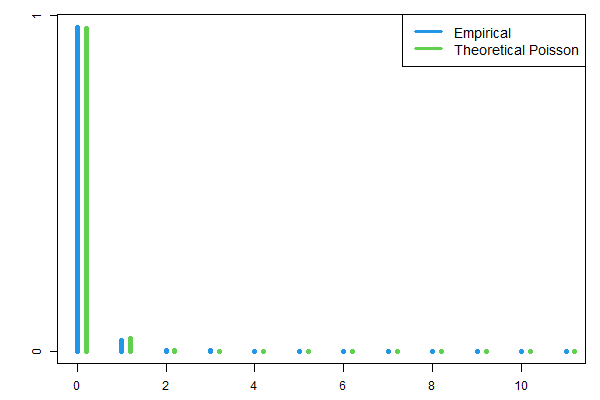
\includegraphics[scale = 0.5]{"../Code & Data/Poisson.png"}
	\label{PoissonGraph}
	\caption{Probability mass of fatal car accidents and theoretical Poisson distribution}
\end{figure}

